
\begin{tabular}{p{7cm}p{4.5cm}p{5cm}}
	Kompensation mit C &
    	\begin{minipage}{4cm}
        	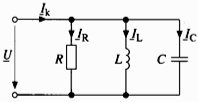
\includegraphics[width=3.5cm]{bilder/Parallelkompensation.png}
        \end{minipage} & 
		Der Kondensator wird parallel dazu geschalten \\ \\
	Zeigerdiagramme Kompensation &
		\begin{minipage}{4.5cm}
        	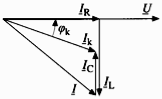
\includegraphics[width=3.5cm]{bilder/Blindstromkompensation.png}
        \end{minipage} &
		\begin{minipage}{4.5cm}
        	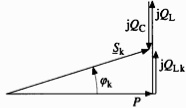
\includegraphics[width=3.5cm]{bilder/Blindleistungskompensation.png}
        \end{minipage} \\ \\
	Neue (kompensierte) Blindleistung &
		$Q_{Lk} = P \cdot \tan{\varphi_k}$ \\
	Blindleistung des Kondensators &
		$Q_C = Q_{Lk} - Q_L$ \\
	Kapazität des Kondensators &
		$C = \frac{Q_C}{\omega U^2}$ \\	
	\end{tabular}